What is tau identification:
- Process of taking reconstructed \tauhadvis candidates and distinguishing their originate
- Predominately sources of \faketauhadvis are quark- or gluon-initiated jets and electrons.
- Here focus on the first source of \faketauhadvis

(Recurrent) neural network-based method:
- Previously boosted decision tree using high-level variables
- Using neural networks to combine high-level information with
low-level information in the form of sequences of tracks and clusters
associated to \tauhadvis candidates.

The identification method is a continuation of the method proposed in
Ref.~\cite{cdeutsch-master} and was published as
Ref.~\cite{ATL-PHYS-PUB-2019-033} with the ATLAS collaboration.

The method described in this chapter is adopted by the ATLAS
collaboration as the recommended \tauid algorithm for analyses using
the \SI{139}{\per\femto\barn} $pp$-collision dataset recorded with the
ATLAS detector during Run~2 of the LHC.

Sections


\section{Introduction}

Tau lepton

Features of hadronic \tauhad decays and how they compare to \tauhad faked by jets

BDT approach and input variables


Motivated by RNNIP: \cite{ATL-PHYS-PUB-2017-003}


\section{Simulated Event Samples}

Training setup, i.e.\ samples (dijet \& $\gamma^*$)

Use as source of \tauhadvis candidates.

Reweighting of (fake) \tauhad \pT


\section{Tau Reconstruction and Identification}

\section{Tau Identification with Recurrent Neural Networks}

\subsection{Input Variables}

\begin{table}[htbp]
  \centering

  \caption{Input variables. Adopted from
    Ref.~\cite{ATL-PHYS-PUB-2019-033}.}%
  \label{tab:tauid_input_variables}

  \renewcommand{\arraystretch}{1.2}

\begin{tabular}{clccp{10.5cm}}
  \toprule
  & Observable & 1-prong & 3-prong & Description \\
  \midrule
  \parbox[t]{2mm}{\multirow{11}{*}{\rotatebox[origin=c]{90}{High-level inputs}}}
  & $p_\text{T}$ & \checkmark & \checkmark
  & Calorimeter-based estimate of \tauhadvis candidate \pT. \\

  & $f_\text{cent}$                & \checkmark & \checkmark
  & Ratio of \ET deposited in calorimeter cells (at EM scale) in cones of $\Delta R < 0.1$ and $\Delta R < 0.2$ about the \tauhadvis axis. \\

  & $f_\text{leadtrack}^{-1}$      & \checkmark & \checkmark
  & Ratio of \ET deposited in calorimeter cells (at EM scale) in a cone of $\Delta R < 0.2$ about the \tauhadvis axis and the \pT of the \pT-leading \emph{core} track. \\

  & $\Delta R_\text{max}$          & \checkmark & \checkmark
  & Maximum $\Delta R$ between core tracks and the \tauhadvis axis. \\

  & $|S_\text{leadtrack}|$         & \checkmark &
  & Transverse impact parameter significance of the \pT-leading track. \\

  & $S_\text{T}^\text{flight}$     &           & \checkmark
  & Transverse flight path significance. \\

  & $f_\text{iso}^\text{track}$    & \checkmark & \checkmark
  & Ratio of scalar sum of \pT of \emph{isolation} tracks and scalar sum of \pT of \emph{core} and \emph{isolation} tracks. \\

  & $f_\text{track}^\text{EM}$     & \checkmark & \checkmark
  & Ratio of the energy in EM clusters$^\dagger$ and the scalar sum of momenta of \emph{core} tracks. \\

  & $p_\text{T}^\text{EM+track}/\pT$ & \checkmark & \checkmark
  & \pT of the \tauhadvis estimated from the momenta of \emph{core} tracks and the two most energetic EM clusters$^\dagger$ divided by the \pT of the calorimetric measurement. \\

  & $m^\text{EM+track}$            & \checkmark & \checkmark
  & Invariant mass of the system of \emph{core} tracks and the two most energetic EM clusters$^\dagger$. \\

  & $m^\text{track}$               &           & \checkmark
  & Invariant mass of the system of \emph{core} tracks. \\
  \midrule
  \parbox[t]{2mm}{\multirow{9}{*}{\rotatebox[origin=c]{90}{Track inputs}}}
  & $p_\text{T}^\text{seed jet}$ & \checkmark & \checkmark
  & \pT of the jet seeding the \tauhadvis candidate. \\

  & $p_\text{T}^\text{track}$    & \checkmark & \checkmark
  & \pT of the track. \\

  & $\Delta\eta^\text{track}$    & \checkmark & \checkmark
  & Difference in $\eta$ between track and \tauhadvis axis. \\

  & $\Delta\phi^\text{track}$    & \checkmark & \checkmark
  & Angle between track and \tauhadvis axis in the transverse plane. \\

  & $|d_0^\text{track}|$         & \checkmark & \checkmark
  & Absolute value of the transverse track impact parameter. \\

  & $|z_0^\text{track} \sin\theta|$ & \checkmark & \checkmark
  & Absolute value of the product of longitudinal track impact parameter and sine of the polar angle of the track. \\

  & $N_\text{IBL hits}$   & \checkmark & \checkmark
  & Number of hits on the track in the IBL. \\

  & $N_\text{Pixel hits}$ & \checkmark & \checkmark
  & Number of hits on the track in pixel detector layers. \\

  & $N_\text{SCT hits}$   & \checkmark & \checkmark
  & Number of hits on the track in SCT layers. \\

  \midrule
  \parbox[t]{2mm}{\multirow{7}{*}{\rotatebox[origin=c]{90}{Cluster inputs}}}
  & $p_\text{T}^\text{jet seed}$ & \checkmark & \checkmark
  & \pT of the jet seeding the \tauhadvis candidate. \\

  & $E_\text{T}^\text{cluster}$ & \checkmark & \checkmark
  & \ET of the cluster. \\

  & $\Delta\eta^\text{cluster}$      & \checkmark & \checkmark
  & Difference in $\eta$ between cluster and \tauhadvis axis. \\

  & $\Delta\phi^\text{cluster}$      & \checkmark & \checkmark
  & Angle between cluster and \tauhadvis axis in the transverse plane. \\

  & $\lambda_\mathrm{cluster}$             & \checkmark & \checkmark
  & Longitudinal distance of the cluster barycentre from the calorimeter front face. \\

  & $\langle \lambda_\mathrm{cluster}^2\rangle$ & \checkmark & \checkmark
  & Second longitudinal cluster moment. \\

  & $\langle r_\mathrm{cluster}^2\rangle$             & \checkmark & \checkmark
  & Second radial cluster moment. \\
  \bottomrule
\end{tabular}

%%% Local Variables:
%%% mode: latex
%%% TeX-master: "../phd_thesis"
%%% End:

\end{table}

\subsection{Network Architecture}

\begin{figure}[htbp]
  \centering

  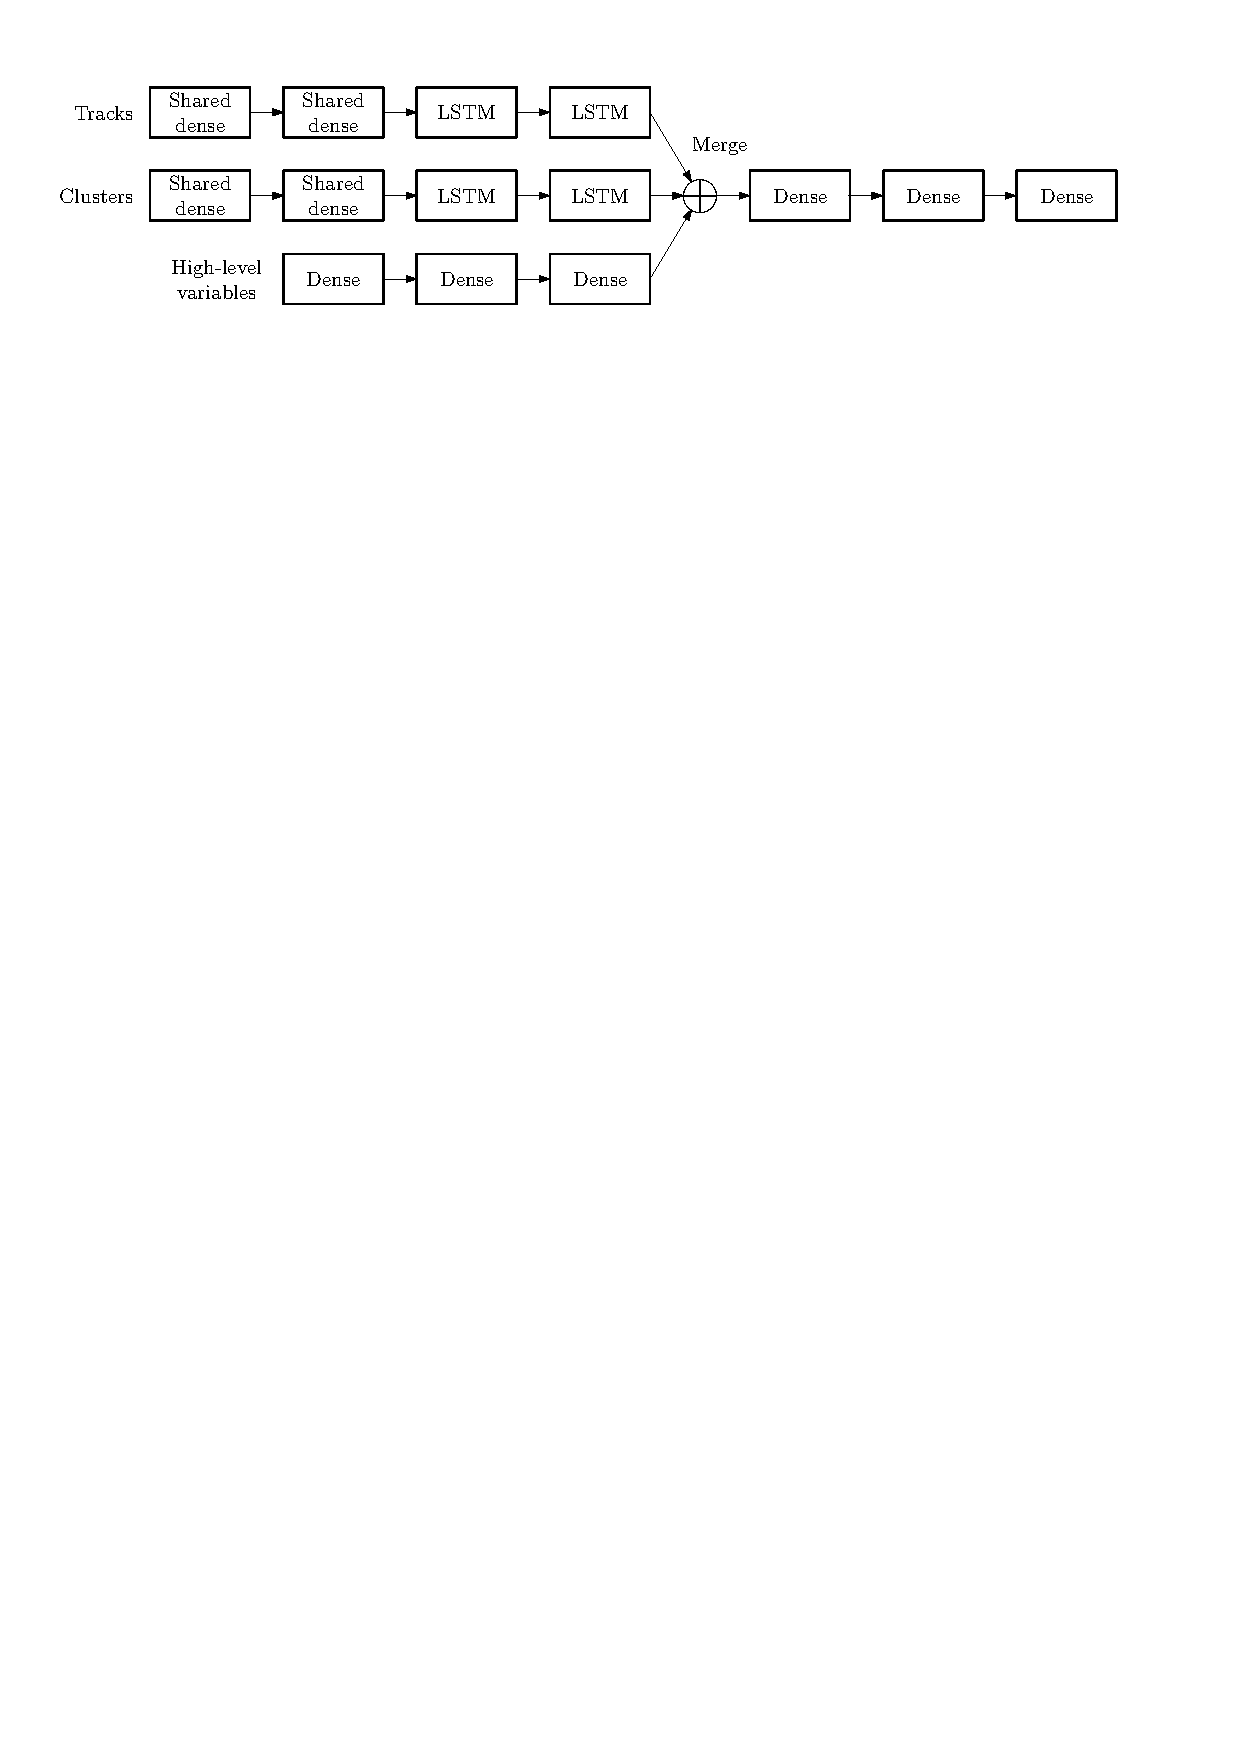
\includegraphics[width=0.95\textwidth]{tauid/pubnote/rnn_network_architecture}

  \caption{Network Architecture of the RNN \tauhad-identification
    algorithm \cite{ATL-PHYS-PUB-2019-033}}
  \label{fig:tauid_network_architecture}
\end{figure}

\subsection{Training and evaluation}

Keras Tensorflow lwtnn \cite{lwtnn,keras,tensorflow2015-whitepaper,lstm}


\subsection{Working Point Definition}


\section{Tau Identification Performance}

\begin{figure}[htbp]
  \centering

  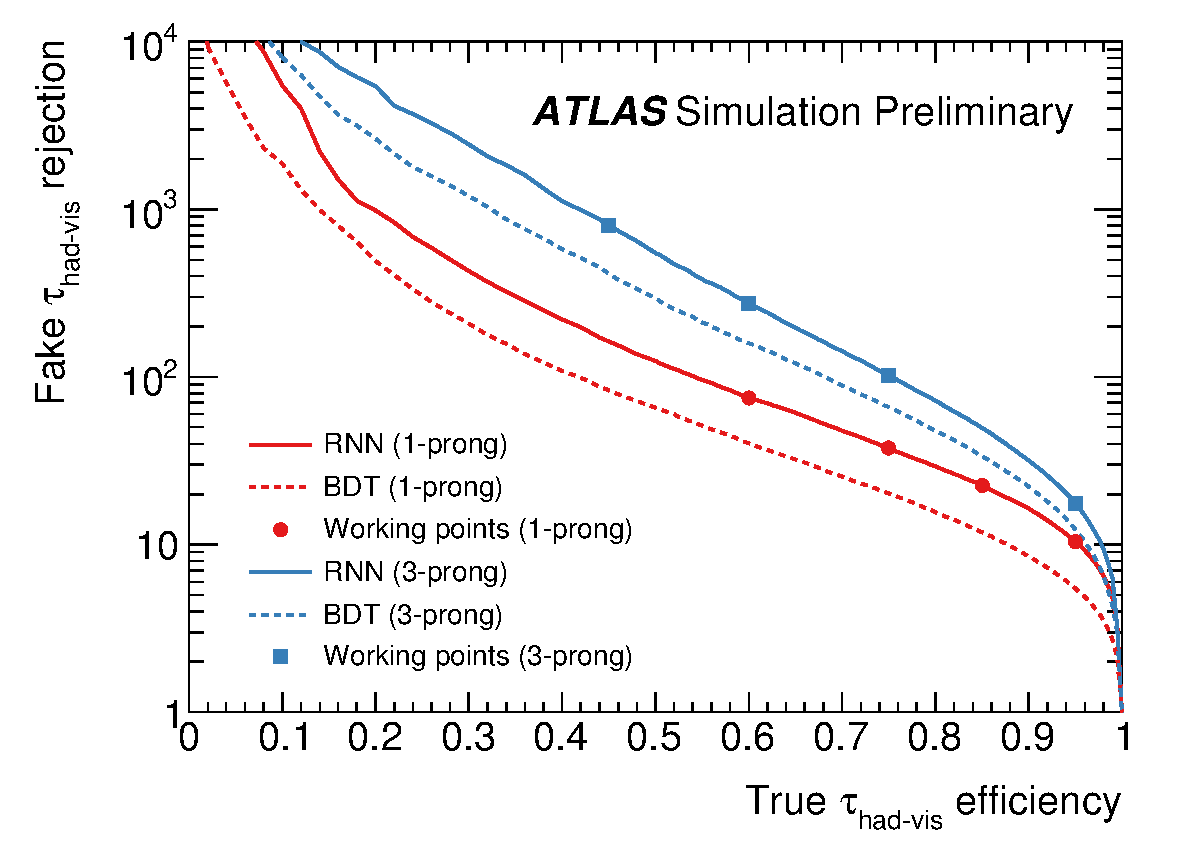
\includegraphics[width=0.6\textwidth]{tauid/pubnote/rnn_bdt_roc}

  \caption{Receiver operating characteristic of the RNN
    \tauhad-identification algorithm \cite{ATL-PHYS-PUB-2019-033}}
  \label{fig:tauid_rnn_bdt_roc_comparison}
\end{figure}


\begin{table}
  \centering

  \caption{List of defined working points with fixed true \tauhadvis
    selection efficiencies and the corresponding background rejection
    factors for misidentified \tauhadvis in dijet events for the BDT
    and RNN classifiers. Adapted from~\cite{ATL-PHYS-PUB-2019-033}.}%
  \label{tab:rnn_wps}

  \begin{tabular}{lcccccc}
    \toprule
                  & \multicolumn{2}{c}{Signal efficiency} & \multicolumn{2}{c}{Background rejection (BDT)} & \multicolumn{2}{c}{Background rejection (RNN)} \\
    Working point  & 1-prong & 3-prong & 1-prong & 3-prong & 1-prong & 3-prong \\
    \midrule
    Tight          & 60\%    & 45\%    & 40      & 400  & 70   & 700 \\
    Medium         & 75\%    & 60\%    & 20      & 150  & 35   & 240 \\
    Loose          & 85\%    & 75\%    & 12      & 61   & 21   & 90  \\
    Very loose     & 95\%    & 95\%    & 5.3     & 11.2 & 9.9  & 16  \\
    \bottomrule
  \end{tabular}
\end{table}

\subsection{Use at the HLT?}

\cite{ATL-DAQ-PUB-2019-001}


\section{Conclusion and Outlook}

To be replaced by ``deep sets'' (permutation invariance). Based on the
same idea and same expected performance but significantly improved
training and prediction time.

%%% Local Variables:
%%% mode: latex
%%% TeX-master: "../../phd_thesis"
%%% End:
